\chapter{Aplikacja Mobilna do Monitorowania Czasu Reakcji}
\section{Cel i funkcje aplikacji mobilnej}
Aplikacja mobilna została zaprojektowana i wykonana, w celu precyzyjnego pomiaru czasu reakcji, oferując trzy poziomy pomiarowe dostosowane do różnych stopni trudności. Na pierwszym poziomie, łatwym, osoba badana musi wybrać guzik o kolorze identycznym z prezentowanym kolorem. W poziomie trudnym prezentowany kolor różni się od koloru guzika, który użytkownik musi wybrać. Najwyższy poziom trudności, zwany bardzo trudnym, utrzymuje zasadę poziomu trudnego, jednak aktywuje również dźwięk o charakterze drażniącym.

Podczas pomiaru, osoba badana widzi jeden z czterech prezentowanych kolorów, a jej zadaniem jest jak najszybsze wybranie guzika odpowiadającego temu kolorowi. Aplikacja precyzyjnie mierzy czas od chwili wyświetlenia koloru do momentu kliknięcia, co pozwala określić czas reakcji. Wyniki pomiarów są zapisywane, a każdy pomiar jest przypisany do nazwy wprowadzonej przed rozpoczęciem pomiaru, umożliwiając łatwe powiązanie wyników z konkretnym uczestnikiem badania.

Aplikacja ma zastosowanie w badaniach nad wpływem niskiego poziomu tlenu na czas reakcji człowieka. Zaprojektowana jest z myślą o dalszych badaniach, gdzie możliwe będzie zbadanie, jak warunki niskiego tlenu wpływają na szybkość reakcji użytkownika. Ta funkcjonalność pozwala na kompleksową analizę reakcji na bodźce wizualne i dźwiękowe, a zebrane dane mogą stanowić istotny wkład w zrozumienie wpływu warunków środowiskowych na funkcje poznawcze człowieka.

\section{Architektura aplikacji}
Do implementacji struktury aplikacji mobilnej, wykorzystano architekturę Model-Widok-Prezenter (MVP) . Architektura MVP jest rozwiązaniem, które doskonale sprawdza się w projektach wymagających jasnego podziału odpowiedzialności pomiędzy warstwami oraz zapewniających elastyczność i łatwość testowania. 
\begin{figure}[!htb]
    \centering
    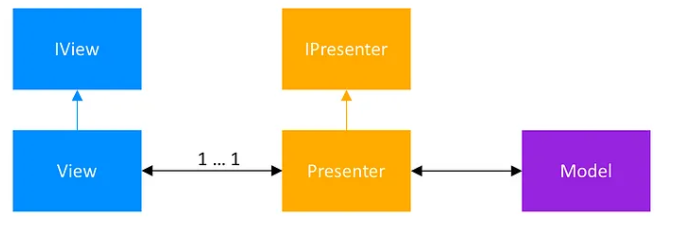
\includegraphics[width=.9\linewidth]{mvp_model.png}
    \caption{Wzorzec MVP - Model View Presenter~\cite{MVP}}
\end{figure}

\subsection{Warstwy aplikacji}
Architektura MVP dzieli strukturę aplikacji na trzy główne komponenty: 
\begin{itemize}
    \item \textbf{Model:} Odpowiada za reprezentację danych oraz logikę biznesową. W wykorzystywanej aplikacji model zawiera logikę związaną z pomairem czasu reakcji, gromadzeniem wyników i komunikację z bazą danych.
    \item \textbf{Widok:} Odpowiada za prezentację danych użytkownikowi oraz obsługe interakcji. Elementy interfejsu użytkownika, takie jak ekran pomiaru czasu reakcji w różnych poziomach trudności składają się na elementy Widoku.
    \item \textbf{Prezenter:} Pośredniczy pomiędzy modelem a widokiem, przekazując dane oraz sterując logiką biznesową. W przedstawionej implementacji prezenter zarządza procesem pomiaru czasu reakcji, obsługą interakcji użytkownika oraz aktualizacją danych modelu.
\end{itemize}

\section{Użyte technologie}
Aplikacja mobilna wykorzystuje zaawansowane technologie programistyczne, bazy danych i platformy wspomagające analizę czasu reakcji. Wykorzystanie wspomnianych technologii stanowi integralną część projektu, umożliwiającą nie tylko efektywne monitorowanie parametrów fizjologicznych, ale także zapewniającą skalowalność i łatwą dostępność danych dla analizy i interpretacji wyników badań. Poniżej przedstawiono kluczowe elementy technologiczne zastosowane w aplikacji:
\begin{itemize}
    \item Android Studio i Java: Aplikacja mobilna została profesjonalnie opracowana w środowisku Android Studio, wykorzystując język programowania Java. Android Studio, będące oficjalnym narzędziem programistycznym dla platformy Android, dostarcza efektywnego środowiska do skutecznej pracy nad projektami, zapewniając jednocześnie intuicyjny interfejs użytkownika.
    \item Firebase: W celu trwałego przechowywania i zarządzania danymi aplikacji, zdecydowano się na wykorzystanie platformy Firebase, kompleksowej usługi od Google. Wykorzystanie Firebase Realtime Database \cite{firebase} umożliwiło składowanie danych dotyczących czasu reakcji, saturacji krwi i fali tętna. Oferuje ona synchronizację w czasie rzeczywistym, co jest kluczowe dla dynamicznych badań.
    \item Gradle: System budowania projektu oparty na Gradle został zastosowany dla efektywnego zarządzania zależnościami, konfiguracją i budowaniem aplikacji. Gradle ułatwia integrację różnych modułów, w tym Firebase, przyczyniając się do płynnego procesu tworzenia i aktualizacji projektu.
\end{itemize}
\section{Komponenty kluczowe}
\subsection{Interfejs użytkownika}
Interfejs użytkownika (UI) to kluczowy element aplikacji, umożliwiający użytkownikowi intuicyjne korzystanie z funkcji pomiaru czasu reakcji. UI zaprojektowano w sposób ergonomiczny, zgodnie z zasadami designu interaktywnego, aby dostarczyć użytkownikowi intuicyjnego i przyjemnego doświadczenia.

Strategiczne rozmieszczenie guzików na stronie startowej ma na celu zminimalizowanie liczby kroków potrzebnych do dostępu do kluczowych funkcji aplikacji. Atrakcyjne logo oraz czytelne, estetycznie wykonane guziki są integralną częścią zapewnienia przyjemnego i intuicyjnego doświadczenia użytkownika podczas korzystania z aplikacji, co jest istotne dla celów badawczych oraz późniejszej analizy wyników pomiarów.
\begin{figure}[!htb]
    \centering
    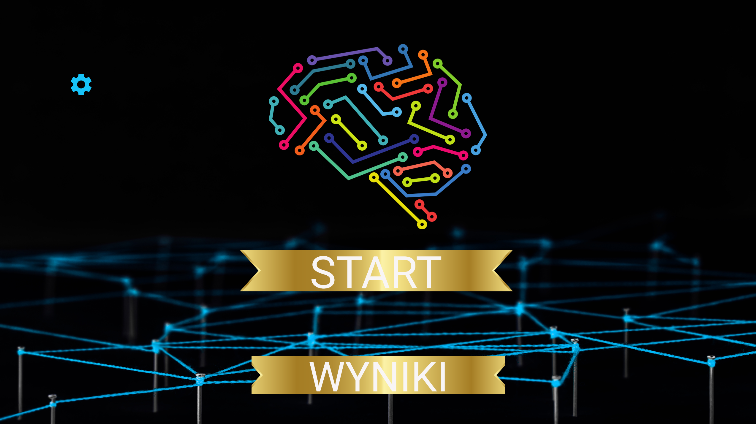
\includegraphics[width=.9\linewidth]{ekran_startowy.png}
    \caption{Widok ekranu startowego aplikacji}
\end{figure}

Po naciśnięciu przycisku START, użytkownik przechodzi do ekranu wyboru poziomu trudności. To kluczowe ogniwo aplikacji, które umożliwia spersonalizowaną adaptację pomiarów czasu reakcji do umiejętności i oczekiwań użytkownika. Na tym ekranie użytkownik ma do wyboru trzy różne poziomy trudności, które zostały opisane powyżej.
\begin{figure}[!htb]
    \centering
    
\includegraphics[width=.9\linewidth]{ekran_poziomu.png}
    \caption{Widok ekranu wyboru poziomu}
\end{figure}

Po wyborze poziomu trudności użytkownik przechodzi do kolejnego etapu, gdzie wprowadza imię osoby biorącej udział w badaniu. To personalizuje pomiar i umożliwia identyfikację wyników. Po wpisaniu imienia użytkownik przystępuje do właściwego badania, które jest centralnym punktem aplikacji.

Na środku ekranu użytkownikowi prezentowany jest jeden z czterech losowo wybranych kolorów: żółty, czerwony, niebieski, zielony. Kolory te są prezentowane w sposób losowy, co zwiększa trudność i różnorodność pomiarów. Jednocześnie na górze ekranu widoczny jest stoper, który precyzyjnie mierzy czas od ostatniego wyboru koloru.

\begin{figure}[!htb]
    \centering
    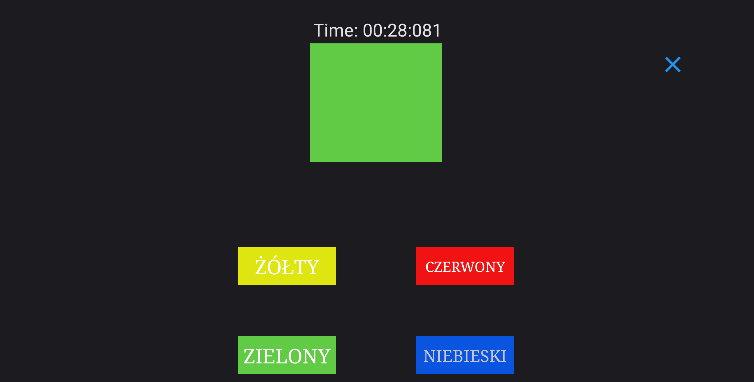
\includegraphics[width=.9\linewidth]{ekran_badania.png}
    \caption{Widok ekranu badania}
\end{figure}
\subsection{Transparentność kodu}
Logika działania aplikacji bejmuje wszystkie procesy i algorytmy związane z pomiarami czasu reakcji oraz interakcjami z użytkownikiem. Prezenter pełni kluczową rolę w zarządzaniu logiką działania, kontrolując sekwencję pomiarów, obsługując interakcje użytkownika i komunikując się z modelem oraz bazą danych. 

Cały kod źródłowy aplikacji został udostępniony publicznie na platformie GitHub~\cite{github}, co umożliwia pełną transparentność, współpracę oraz dostępność dla społeczności programistycznej. W repozytorium znajdują się wszystkie niezbędne pliki, w tym strukturę projektu, kod, pliki konfiguracyjne oraz dodatkowe zasoby. Ze względu na rozmiar kodu i złożoność jego struktury, omawianie go w ramach pracy byłoby nieefektywne. Zachęcam do zapoznania się z kodem na platformie GitHub, gdzie każdy fragment jest starannie udokumentowany, a kod głównego działania aplikacji stanowi serce projektu. Link do repozytorium jest dostępny w źródłach pracy.
\subsection{Baza danych}
Do przechowywania wyników uzyskanych podczas badań została wykorzystana zaawansowana platforma Firebase. Struktura bazy danych została starannie zaprojektowana, aby efektywnie gromadzić i udostępniać informacje na temat czasu reakcji użytkowników.

\begin{figure}[!htb]
    \centering
    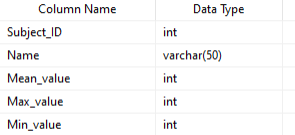
\includegraphics[width=.9\linewidth]{baza_danych.png}
    \caption{Schemat bazy danych}
\end{figure}

Dzięki tej strukturze, każde badanie jest identyfikowane przez nazwę, a wyniki związane z danym badaniem są przechowywane w odpowiednich gałęziach bazy danych. Poszczególne wyniki zawierają informacje o imieniu osoby badanej, jak również o minimalnym, maksymalnym oraz średnim czasie reakcji.
Wyniki uzyskane w trakcie badania są dostępne zarówno dla osób badanych, które mogą natychmiast otrzymać informacje o swoim czasie reakcji, jak i dla osób analizujących, które mają dostęp do wyników w późniejszym czasie. To zapewnia kompleksową analizę i interpretację zebranych danych.
\begin{figure}[!htb]
    \centering
    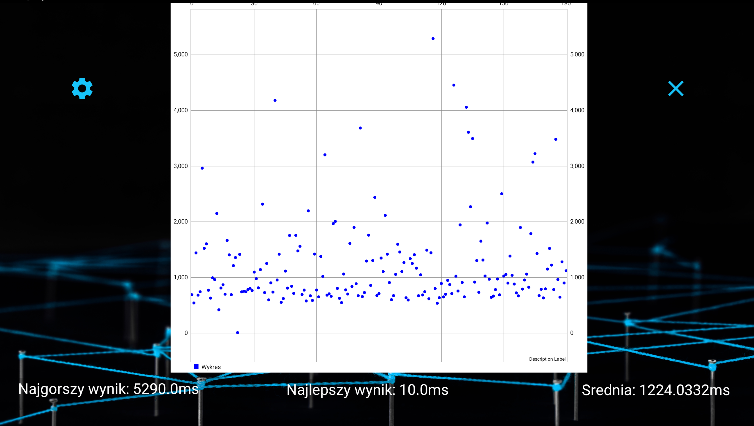
\includegraphics[width=.9\linewidth]{ekran_wyniki.png}
    \caption{Widok ekranu wyników}
\end{figure}

Zintegrowane działanie tych trzech kluczowych komponentów zapewnia nie tylko płynne i precyzyjne pomiary czasu reakcji, ale również umożliwia gromadzenie danych w sposób, który będzie fundamentalny dla przyszłych badań nad wpływem niskiego poziomu tlenu na czas reakcji ludzi, zwłaszcza w kontekście warunków ekstremalnych, takich jak w górach.
\section{Testowanie}
W kontekście testowania aplikacji mobilnej do monitorowania czasu reakcji, przeprowadzono szereg różnorodnych testów \cite{testy}, obejmujących kluczowe aspekty funkcjonalne, interfejs użytkownika oraz wydajność. Szczegółowy opis przeprowadzonych testów:
\begin{itemize}
    \item \textbf{Testy Jendostkowe: } Sprawdzenie poprawność działania poszczególnych funkcji, takich jak generowanie losowego koloru, pomiar czasu reakcji czy zapis wyników oraz upewnienie się, że funkcje obsługują różne sceraiusze. w tym poprawne i niepoprawne dane wejściowe.
    \item \textbf{Testy Integracyjne: } Upewnienie się, że dane są przekazywane i odbierane poprawnie między interfejsem użytkownika a logiką biznesową.
    \item \textbf{ Testy Interfejsu Użytkownika: } Przetestowano interfejs użytkownika pod kątem intuicyjności i łatwości obsługi oraz zapewnienie, że interfejs jest responsywny na różnych urządzeniach i rozdzielczościach
    \item \textbf{Testy Bazy Danych: } Sprawdzenie poprawności zapisywania i odczytywania danych z bazy Firebase
\end{itemize}
\section{Mozliowść rozwoju}
Aplikacja do monitorowania czasu reakcji stanowi dynamiczne narzędzie badawcze, oferujące rozległy potencjał rozwoju. Możliwość rozszerzenia poziomów trudności wzbogaci badania nad reakcjami fizjologicznymi, umożliwiając prowadzenie zaawansowanych analiz. Funkcja personalizacji pozwoli użytkownikom dostosować ustawienia badań do swoich preferencji, co wpłynie na bardziej zindywidualizowane i trafne wyniki. Zaawansowane narzędzia analizy statystycznej dodadzą głębszego kontekstu zrozumienia wyników badań, podnosząc jakość analizy. Dodatkowo, funkcje powiadomień i motywacji zwiększą zaangażowanie użytkowników, sprzyjając regularnym badaniom.

Rozwinięcie aplikacji o współpracę zespołową umożliwi analizę grupową i agregację wyników, co może przyczynić się do bardziej kompleksowych wniosków. Integracja z urządzeniami noszonymi, takimi jak smartwatche, pozwoli na ciągłe monitorowanie parametrów fizjologicznych, co jest istotne w kontekście długotrwałych badań. Optymalizacja interfejsu użytkownika i estetyczne doświadczenie są kluczowe dla zadowolenia i skuteczności użytkowania. Współpraca z naukowcami i instytucjami badawczymi otworzy drzwi do interdyscyplinarnych analiz, poszerzając zakres zastosowań aplikacji.

Przeniesienie aplikacji na różne platformy mobilne, takie jak iOS, zapewniłoby szeroką dostępność, dotarcie do szerszego grona użytkowników oraz zwiększenie wpływu aplikacji na społeczność badawczą. Wprowadzenie dodatkowych warstw bezpieczeństwa, takich jak szyfrowanie danych, podniesie poziom ochrony prywatności użytkowników, co jest kluczowe w kontekście przechowywania danych medycznych. Całkowity rozwój aplikacji w oparciu o te kierunki przysłuży się jej popularności, ułatwiając jednocześnie zaawansowane badania w monitorowaniu parametrów fizjologicznych.